\chapter{WMC Without Parameter Variables}\label{chapter:wmc2}

\section{Introduction}

Recall that in \cref{chapter:wmc1} we examined WMC from a measure-theoretic
perspective and found that---due to the rigidity of the standard
formulation---WMC encodings usually contain many superfluous variables. This
observation inspired an encoding for Bayesian networks that alleviates the
issue. In this chapter, we continue to tackle the subject of superfluous
parameter variables but take the solution a few steps further.

If WMC is not the right format for probabilistic inference and other
sum-of-products computations, what could be a better alternative? As many WMC
inference algorithms \citep{DBLP:conf/ecai/Darwiche04,DBLP:conf/ijcai/OztokD15}
work by compilation to tractable representations such as arithmetic circuits,
deterministic, decomposable negation normal form
\citep{DBLP:journals/jancl/Darwiche01}, and sentential decision diagrams (SDDs)
\citep{DBLP:conf/ijcai/Darwiche11}, perhaps parameter variables could be avoided
via direct compilation to a more convenient representation. Direct compilation
of Bayesian networks to SDDs has been investigated
\citep{DBLP:conf/ecsqaru/ChoiKD13}. However, SDDs only support weights on
literals, and so are not expressive enough to avoid the issue.
\Citet{DBLP:conf/uai/GogateD10} propose a format based on weighted clauses and
probabilistic semantics inspired by Markov networks. However, with a new
representation comes the need to invent new encodings and inference algorithms.
Moreover, to the best of our knowledge, neither approach
\citep{DBLP:conf/ecsqaru/ChoiKD13,DBLP:conf/uai/GogateD10} has a publicly
available implementation.

In this work, we introduce a new computational problem called
\emph{pseudo-Boolean projection} (PBP)---a generalisation of the conditional
weights approach proposed in \cref{chapter:wmc1}. Recent WMC algorithms based on
pseudo-Boolean function manipulation---namely, \textsc{ADDMC}
\citep{DBLP:conf/aaai/DudekPV20} and \textsc{DPMC}
\citep{DBLP:conf/cp/DudekPV20}---can easily be adapted to the new format. In
contrast to our previous work, instead of inventing new encodings, we show how
every WMC problem instance can be transformed to PBP and identify conditions
under which this transformation can remove parameter variables. Four out of the
five known WMC encodings for Bayesian networks
\citep{DBLP:conf/ecai/BartKLM16,DBLP:conf/ijcai/ChaviraD05,DBLP:conf/sat/ChaviraD06,DBLP:conf/kr/Darwiche02,DBLP:conf/aaai/SangBK05}
can indeed be simplified in this manner. We are able to eliminate
\SI{43}{\percent} of variables on average and up to \SI{99}{\percent} on some
instances. This transformation enables two encodings that were previously
incompatible with most WMC algorithms (due to using a different formulation of
WMC \citep{DBLP:conf/ijcai/ChaviraD05,DBLP:conf/sat/ChaviraD06}) to be run with
\textsc{ADDMC} and \textsc{DPMC} and results in a significant performance boost
for one other encoding, making it about three times faster than the state of the
art. Finally, our theoretical contributions result in a convenient algebraic way
of reasoning about two-valued pseudo-Boolean functions and position WMC
encodings on common ground, identifying their key properties and assumptions.

% Specifically, direct compilation
% from Bayesian networks to SDDs \citep{DBLP:conf/ecsqaru/ChoiKD13} and from
% structured Bayesian networks (i.e., a generalisation of Bayesian networks) to
% probabilistic SDDs \citep{shen2020modeling} have been considered.

% * SDD compilation still has parameter variables
% 1) However, no conversion algorithms from either WMC or probabilistic models
% are provided.
% Since we present a WMC to PBP algorithm, we don't need to invent new
% encodings for each problem and we can benefit from all the good ideas that
% went into designing WMC encodings
% 3) Instead of combining techniques from older WMC algorithms like they did, we
% use a much more recent WMC solver that is shown to...
% 3) We benefit from a decade of research in WMC inference and, specifically, 
% 4) We are not restricted to clauses and probabilistic semantics
% 5) We identify conditions and describe an algorithm for transforming any WMC
% instance into PBP

\section{Redefining WMC}

Since the goal of this chapter is to generalise WMC in a way that eliminates the
redundant parameter variables, in this section we redefine WMC in a way that
explicitly partitions all variables into parameter and indicator variables. We
also formalise a variant of WMC that has been implicitly used by
\citet{DBLP:conf/ijcai/ChaviraD05,DBLP:conf/sat/ChaviraD06}.

In this chapter, we denote interpretations (and models) of a propositional
formula as subsets of the set of variables. These variables are implicitly
mapped to \texttt{true} whereas all other variables are mapped to
\texttt{false}. The \emph{cardinality} of a model is then the cardinality of
this set.

\begin{example}
  Let $\phi = (\neg a \lor b) \land a$ be a propositional formula over variables
  $a$ and $b$. Then $\{\, a, b \,\}$ (i.e.,
  $\{\, a \mapsto \texttt{true}, b \mapsto \texttt{true} \,\}$) is a model of
  $\phi$ (written $\{\, a, b \,\} \models \phi$), and it has cardinality two.
\end{example}

\begin{definition}[WMC]\label{def:wmc}
  A \emph{WMC instance} is a tuple $(\phi, X_I, X_P, w)$, where $X_I$ is the set
  of \emph{indicator variables}, $X_P$ is the set of \emph{parameter variables}
  (with $X_I \cap X_P = \emptyset$), $\phi$ is a propositional formula in CNF
  over $X_I \cup X_P$, and
  $w\colon X_I \cup X_P \cup \{\, \neg x \mid x \in X_I \cup X_P \,\} \to \mathbb{R}$
  is a \emph{weight function} such that $w(x) = w(\neg x) = 1$ for all
  $x \in X_I$. The \emph{answer} of the instance is
  $\sum_{Y \models \phi} \prod_{Y \models l} w(l)$.
\end{definition}

In practice, we identify this partition of variables in one of two ways. If an
encoding is generated by \textsc{Ace}\footnote{\textsc{Ace}
  \citep{DBLP:journals/ai/ChaviraD08} implements most of the Bayesian network
  encodings and can also be used for compilation (and thus inference). It is
  available at \url{http://reasoning.cs.ucla.edu/ace/}.}, then variable types
are explicitly identified in a file generated alongside the encoding. Otherwise,
we take $X_I$ to be the set of all variables $x$ such that
$w(x) = w(\neg x) = 1$. Next, we formally define another variant of WMC.

\begin{definition}
  Let $\phi$ be a formula over a set of variables $X$. Then $Y \subseteq X$ is a
  \emph{minimum-cardinality model} of $\phi$ if $Y \models \phi$ and $|Y| \le
  |Z|$ for all $Z \models \phi$.
\end{definition}

\begin{definition}[Minimum-cardinality WMC]\label{def:mcwmc}
  A \emph{minimum-cardinality WMC} instance consists of the same tuple as a WMC
  instance, but its \emph{answer} is defined to be
  \[
  \sum_{Y \models \phi\text{,}|Y| = k} \prod_{Y \models l} w(l)
  \]
  (where $k = \min_{Y \models \phi} |Y|$) if $\phi$ is satisfiable, and zero otherwise.
\end{definition}

\begin{example}\label{example:1}
  Let
  $\phi = (x \lor y) \land (\neg x \lor \neg y) \land (\neg x \lor p) \land (\neg y \lor q) \land x$,
  $X_I = \{\, x, y \,\}$, $X_P = \{\, p, q \,\}$, $w(p) = 0.2$, $w(q) = 0.8$,
  and $w(\neg p) = w(\neg q) = 1$. Then $\phi$ has two models: $\{\, x, p \,\}$
  and $\{\, x, p, q \,\}$ with weights $0.2$ and $0.2 \times 0.8 = 0.16$,
  respectively. The WMC answer is then $0.2 + 0.16 = 0.36$, and the
  minimum-cardinality WMC answer is $0.2$.
\end{example}

\section{Bayesian Network Encodings}\label{sec:encodings}

Recall that a \emph{Bayesian network} is a directed acyclic graph with random
variables as vertices and edges as conditional dependencies. As is common in
related literature \citep{DBLP:conf/kr/Darwiche02,DBLP:conf/aaai/SangBK05}, we
assume that each variable has a finite number of values. We call a Bayesian
network \emph{binary} if every variable has two values.

WMC is a well-established technique for Bayesian network inference, particularly
effective on networks where most variables have only a few possible values
\citep{DBLP:conf/kr/Darwiche02}. Many ways of encoding a Bayesian network into a
WMC instance have been proposed. \Citet{DBLP:conf/kr/Darwiche02} was the first
to suggest the \texttt{d02} encoding that, in many ways, remains the foundation
behind most other encodings. He also introduced the distinction between
\emph{indicator} and \emph{parameter variables}; the former represent
variable-value pairs in the Bayesian network, while the latter are associated
with probabilities in the conditional probability tables (CPTs). The encoding
\texttt{sbk05} \citep{DBLP:conf/aaai/SangBK05} is the only encoding that
deviates from this arrangement: for each variable in the Bayesian network, one
indicator variable acts simultaneously as a parameter variable.
\Citet{DBLP:conf/ijcai/ChaviraD05} propose \texttt{cd05} where they shift from
WMC to minimum-cardinality WMC because that allows the encoding to have fewer
variables and clauses. In particular, they propose a way to use the same
parameter variable to represent all probabilities in a CPT that are equal and
keep only clauses that `imply' parameter variables (i.e., omit clauses where a
parameter variable implies indicator variables).\footnote{\Cref{example:2}
  demonstrates what we mean by implication clauses.} In their next encoding,
\texttt{cd06}, \citet{DBLP:conf/sat/ChaviraD06} optimise the aforementioned
implication clauses, choosing the smallest sufficient selection of indicator
variables. A decade later, \citet{DBLP:conf/ecai/BartKLM16} present
\texttt{bklm16} that improves upon \texttt{cd06} in two ways. First, they
optimise the number of indicator variables used per Bayesian network variable
from a linear to a logarithmic amount. Second, they introduce a scaling factor
that can `absorb' one probability per Bayesian network variable. However, for
this work, we choose to disable the latter improvement since this scaling factor
is often small enough to be indistinguishable from zero without the use of
arbitrary precision arithmetic, making it completely unusable on realistic
instances. Indeed, the reader is free to check that even a small Bayesian
network with seven mutually independent binary variables, 0.1 and 0.9
probabilities each, is already big enough for the scaling factor to be exactly
equal to zero (as produced by the \texttt{bklm16}
encoder\footnote{\url{http://www.cril.univ-artois.fr/kc/bn2cnf.html}}). We
suspect that this issue was not identified during the original set of
experiments because the authors never looked at numerical answers.

\begin{example} \label{example:2}
  Let $\mathcal{B}$ be a Bayesian network with one variable $X$ which has two
  values $x_1$ and $x_2$ with probabilities $\Pr(X = x_1) = 0.2$ and $\Pr(X =
  x_2) = 0.8$. Let $x, y$ be indicator variables, and $p, q$ be parameter
  variables. Then \cref{example:1} is both the \texttt{cd05} and the
  \texttt{cd06} encoding of $\mathcal{B}$. The \texttt{bklm16} encoding is $(x
  \Rightarrow p) \land (\neg x \Rightarrow q) \land x$ with $w(p) = w(\neg q) =
  0.2$, and $w(\neg p) = w(q) = 0.8$. And the \texttt{d02} encoding is $(\neg x
  \Rightarrow p) \land (p \Rightarrow \neg x) \land (x \Rightarrow q) \land (q
  \Rightarrow x) \land \neg x$ with $w(p) = 0.2$, $w(q) = 0.8$, and $w(\neg p) =
  w(\neg q) = 1$. Note how all other encodings have fewer clauses than
  \texttt{d02}. While \texttt{cd05} and \texttt{cd06} require
  minimum-cardinality WMC to make this work, \texttt{bklm16} achieves the same
  thing by adjusting weights.\footnote{Note that since \texttt{cd05} and
    \texttt{cd06} are minimum-cardinality WMC encodings, they are not supported
    by most WMC algorithms.}
\end{example}

%This additional condition on model
%cardinality becomes necessary because these encodings eliminate clauses of the
%form $p \Rightarrow i$, where $p \in X_P$ is a parameter variable, and $i \in
%X_I$ is an indicator variable. Nonetheless, our transformation algorithm still
%works on such encodings, although the experimental results are discouraging
%because they use approximately twice as many indicator variables. For
%instance, each binary variable of a Bayesian network is encoded using two
%indicator variables while one would suffice.

\section{Pseudo-Boolean Functions}

In this work, we propose a more expressive representation for WMC based on
pseudo-Boolean functions. Since two-valued pseudo-Boolean functions will be used
extensively henceforth, we introduce some new notation. For any propositional
formula $\phi$ over a set of variables $X$ and $p, q \in \mathbb{R}$, let
${[\phi]}^p_q\colon 2^X \to \mathbb{R}$ be the pseudo-Boolean function defined
as
\[
  {[\phi]}^p_q(Y) \coloneqq
  \begin{cases}
    p & \text{if } Y \models \phi \\
    q & \text{otherwise}
  \end{cases}
\]
for any $Y \subseteq X$.

Below we list some properties of the operations on pseudo-Boolean functions that
can be conveniently represented using our syntax. The proofs of all these
properties follow directly from the definitions.

\begin{proposition}[Basic properties]\label{prop:basic}
  For any propositional formulas $\phi$ and $\psi$, and
  $a, b, c, d \in \mathbb{R}$,
  \begin{itemize}
    \item ${[\phi]}^a_b = {[\neg \phi]}^b_a$;
    \item $c + {[\phi]}^a_b = {[\phi]}^{a+c}_{b+c}$;
    \item $c \cdot {[\phi]}^a_b = {[\phi]}^{ac}_{bc}$;
    \item ${[\phi]}^a_b \cdot {[\phi]}^c_d = {[\phi]}^{ac}_{bd}$;
    \item ${[\phi]}^1_0 \cdot {[\psi]}_0^1 = {[\phi \land \psi]}_0^1$.
  \end{itemize}
  And for any pair of pseudo-Boolean functions $f, g \colon 2^X \to \mathbb{R}$
  and $x \in X$, $(fg)|_{x=i} = f|_{x=i} \cdot g|_{x=i}$ for $i = 0, 1$.
\end{proposition}

\begin{remark}
  For convenience, we assume that the domain of a pseudo-Boolean function $f$
  shrinks whenever $f$ is independent of some of the variables (i.e.,
  $f|_{x=0} = f|_{x=1}$) and expand for binary operations to make the domains of
  both functions equal. For instance, let
  ${[x]}_0^1,{[\neg x]}_0^1\colon 2^{\{\, x \,\}} \to \mathbb{R}$ and
  ${[y]}_0^1\colon 2^{\{\, y \,\}} \to \mathbb{R}$ be pseudo-Boolean functions.
  Then ${[x]}_0^1 \cdot {[\neg x]}_0^1$ has $2^\emptyset$ as its domain. To
  multiply ${[x]}_0^1$ and ${[y]}_0^1$, we expand ${[x]}_0^1$ into
  $\left({[x]}_0^1\right)'\colon 2^{\{\, x, y \,\}} \to \mathbb{R}$ which is
  defined as
  $\left({[x]}_0^1\right)'(Z) \coloneqq {[x]}_0^1(Z \cap \{\, x \,\})$ for all
  $Z \subseteq \{\, x, y \,\}$ (and equivalently for ${[y]}_0^1$).
\end{remark}

\section{Pseudo-Boolean Projection}

We introduce a new type of computational problem called \emph{pseudo-Boolean
  projection} based on two-valued pseudo-Boolean functions. While the same
computational framework can handle any pseudo-Boolean functions, two-valued
functions are particularly convenient because \textsc{DPMC}
\citep{DBLP:conf/cp/DudekPV20} can be easily adapted to use them as input. Since
we will only encounter functions of the form ${[\phi]}^a_b$, where $\phi$ is a
conjunction of literals, we can represent it in text as \texttt{w
  $\langle\phi\rangle$ a b} where $\langle\phi\rangle$ is a representation of
$\phi$ analogous to the representation of a clause in the DIMACS CNF format.

\begin{definition}[PBP instance]\label{def:pbp}
  A PBP instance is a tuple $(F, X, \omega)$, where $X$ is the set of variables,
  $F$ is a set of two-valued pseudo-Boolean functions $2^X \to \mathbb{R}$, and
  $\omega \in \mathbb{R}$ is the scaling factor.\footnote{ Adding scaling factor
    $\omega$ to the definition allows us to remove clauses that consist entirely
    of a single parameter variable. The idea of extracting some of the structure
    of the WMC instance into an external multiplicative factor was loosely
    inspired by the \texttt{bklm16} encoding, where it is used to subsume the
    most commonly occurring probability of each CPT
    \citep{DBLP:conf/ecai/BartKLM16}.} Its \emph{answer} is
  $\omega \cdot \left(\exists_X\prod_{f \in F}f\right)(\emptyset)$.
\end{definition}

\subsection{From WMC to PBP}

In this section, we describe an algorithm for transforming WMC instances to the
PBP format while removing all parameter variables. We chose to transform
existing encodings instead of creating a new one to reuse already-existing
techniques for encoding each CPT to its minimal logical representation such as
prime implicants and limited forms of resolution
\citep{DBLP:conf/ecai/BartKLM16,DBLP:conf/ijcai/ChaviraD05,DBLP:conf/sat/ChaviraD06}.
The transformation algorithm works on four out of the five Bayesian network
encodings: \texttt{bklm16} \citep{DBLP:conf/ecai/BartKLM16}, \texttt{cd05}
\citep{DBLP:conf/ijcai/ChaviraD05}, \texttt{cd06}
\citep{DBLP:conf/sat/ChaviraD06}, and \texttt{d02}
\citep{DBLP:conf/kr/Darwiche02}. There is no obvious way to adjust it to work
with \texttt{sbk05} because the roles of indicator and parameter variables
overlap \citep{DBLP:conf/aaai/SangBK05}.

The algorithm is based on several observations that will be made more precise in
\cref{sec:proof}. First, all weights except for $\{\, w(p) \mid p \in X_P \,\}$
are redundant as they either duplicate an already-defined weight or are equal to
one. Second, each clause has at most one parameter variable. Third, if the
parameter variable is negated, we can ignore the clause (this idea comes from
the work of \citet{DBLP:conf/ijcai/ChaviraD05}). Note that while we formulate
our algorithm as a sequel to the WMC encoding procedure primarily because the
implementations of Bayesian network WMC encodings are all closed-source, as all
transformations in the algorithm are local, it can be efficiently incorporated
into a WMC encoding algorithm with no slowdown.

\begin{algorithm}[t]
  \caption{WMC to PBP transformation.}\label{alg:transformation}
  \SetKwFunction{rename}{rename}
  \SetKwProg{Fn}{Function}{:}{}
  \KwData{WMC (or minimum-cardinality WMC) instance $(\phi, X_I, X_P, w)$}
  \KwResult{PBP instance $(F, X_I, \omega)$}
  $F \gets \emptyset$\;
  $\omega \gets 1$\;
  \ForEach{clause $c \in \phi$\label{line:foreach1start}}{
    \uIf{$c \cap X_P = \{\, p \,\}$ for some variable $p$ \textnormal{\textbf{and}} $w(p) \ne 1$}{
      \lIf{$|c| = 1$}{$\omega \gets \omega \times w(p)$}
      \lElse{$F \gets F \cup \left\{\, {\left[ \bigwedge_{l \in c \setminus \{\, p \,\}} \neg l \right]}^{w(p)}_1 \,\right\}$}
    }
    \ElseIf{$\{\, p \mid \neg p \in c \,\} \cap X_P  = \emptyset$}{
      $F \gets F \cup \{\, {[c]}^1_0 \,\}$\;\label{line:foreach1end}
    }
  }
  \ForEach{variable $v \in X_I$ such that $\{\ {[v]}_1^p, {[\neg v]}_1^q \,\} \subseteq F$ for some $p$ and $q$\label{line:foreach2start}}{
    $F \gets F \setminus \{\, {[v]}_1^p, {[\neg v]}_1^q \,\} \cup \{\, {[v]}_q^p \,\}$\;\label{line:foreach2end}
  }
\end{algorithm}

The algorithm is listed as \cref{alg:transformation}. The main part of the
algorithm is the first loop that iterates over clauses. If a clause consists of
a single parameter variable, we incorporate it into $\omega$. If a clause is of
the form $\alpha \Rightarrow p$, where $p \in X_P$, and $\alpha$ is a
conjunction of literals over $X_I$, we transform it into a pseudo-Boolean
function ${[\alpha]}_1^{w(p)}$. If a clause $c \in \phi$ has no parameter
variables, we reformulate it into a pseudo-Boolean function ${[c]}_0^1$.
Finally, clauses with negative parameter literals are omitted.

As all `weighted' pseudo-Boolean functions produced by the first loop are of the
form ${[\alpha]}_1^p$ (for some $p \in \mathbb{R}$ and formula $\alpha$), the
second loop merges two functions into one whenever $\alpha$ is a literal. Note
that taking into account the order in which clauses are typically generated by
encoding algorithms allows us to do this in linear time (i.e., the two mergeable
functions will be generated one after the other).

%\item The second \textbf{foreach} loop can be performed in constant time by
%  representing $\phi'$ as a list and assuming that the two 'clauses' are
%  adjacent in that list (and incorporating it into the first loop).
%\item The $d$ map is constructed in $\mathcal{O}(|X_P|\log|X_P|)$ time (we want
%  to use a data structure based on binary search trees rather than hashing).
%\item \texttt{rename} can be implemented in $\mathcal{O}(\log |X_P|)$ time.

\subsection{Correctness Proofs}\label{sec:proof}

In this section, we outline key conditions that a (WMC or minimum-cardinality
WMC) encoding has to satisfy for \cref{alg:transformation} to output an
equivalent PBP instance. We divide the correctness proof into two theorems:
\cref{thm:correctness2} for WMC encodings (i.e., \texttt{bklm16} and
\texttt{d02}) and \cref{thm:mccorrectness} for minimum-cardinality WMC encodings
(i.e., \texttt{cd05} and \texttt{cd06}). We begin by listing some properties of
pseudo-Boolean functions and establishing a canonical transformation from WMC to
PBP\@.

\begin{theorem}[Early projection
  \citep{DBLP:conf/aaai/DudekPV20,DBLP:conf/cp/DudekPV20}]\label{thm:early}
  Let $X$ and $Y$ be sets of variables. For all pseudo-Boolean functions
  $f\colon 2^X \to \mathbb{R}$ and $g\colon 2^Y \to \mathbb{R}$, if $x \in X
  \setminus Y$, then $\exists_x (f \cdot g) = (\exists_x f) \cdot g$.
\end{theorem}

\begin{lemma}\label{lemma:sum}
  For any pseudo-Boolean function $f\colon 2^X \to \mathbb{R}$, we have that
  $(\exists_X f)(\emptyset) = \sum_{Y \subseteq X} f(Y)$.
\end{lemma}
\begin{proof}
  If $X = \{\, x \,\}$, then
  \[
    (\exists_{x}f)(\emptyset) = (f|_{x=1} + f|_{x=0})(\emptyset) = f|_{x=1}(\emptyset) + f|_{x=0}(\emptyset) = \sum_{Y \subseteq \{\, x \,\}} f(Y).
  \]
  This easily extends to $|X| > 1$ by the definition of projection on sets of
  variables.
\end{proof}

\begin{proposition}\label{prop:equivalence}
  Let $(\phi, X_I, X_P, w)$ be a WMC instance. Then
  \begin{equation}
  \left( \left\{\, {[c]}_0^1 \;\middle|\; c \in \phi \,\right\} \cup \left\{\, {[x]}_{w(\neg x)}^{w(x)} \;\middle|\; x \in X_I \cup X_P \,\right\}, X_I \cup X_P, 1 \right) \label{eq:new_wmc}
  \end{equation}
  is a PBP instance with the same answer (as in \cref{def:wmc,def:pbp}).
\end{proposition}
\begin{proof}
  Let $f = \prod_{c \in \phi} {[c]}_0^1$, and
  $g = \prod_{x \in X_I \cup X_P} {[x]}_{w(\neg x)}^{w(x)}$. Then the WMC answer
  of~\eqref{eq:new_wmc} is
  $(\exists_{X_I \cup X_P} fg)(\emptyset) = \sum_{Y \subseteq X_I \cup X_P} (fg)(Y) = \sum_{Y \subseteq X_I \cup X_P} f(Y)g(Y)$
  by \cref{lemma:sum}. Note that
  \[
    f(Y) =
    \begin{cases}
      1 & \text{if } Y \models \phi, \\
      0 & \text{otherwise},
    \end{cases}
    \quad
    \text{and}
    \quad
    g(Y) = \prod_{Y \models l} w(l),
  \]
  which means that
  $\sum_{Y \subseteq X_I \cup X_P} f(Y)g(Y) = \sum_{Y \models \phi} \prod_{Y \models l} w(l)$
  as required.
\end{proof}

\begin{theorem}[Correctness for WMC]\label{thm:correctness2}
  \Cref{alg:transformation}, when given a WMC instance $(\phi, X_I, X_P, w)$,
  returns a PBP instance with the same answer (as defined in
  \cref{def:wmc,def:pbp}), provided \emph{either} of the two conditions is
  satisfied:
  \begin{enumerate}
    \item for all $p \in X_P$, there is a non-empty family of literals
          ${(l_i)}_{i=1}^n$ such that\label{cond:d02}
          \begin{enumerate}
            \item $w(\neg p) = 1$,
            \item $l_i \in X_I$ or $\neg l_i \in X_I$ for all
                  $i = 1, \dots, n$,\label{condition:equivalence1}
            \item and $\{\, c \in \phi \mid p \in c \text{ or } \neg p \in c \,\} = \left\{\, p \lor \bigvee_{i=1}^n \neg l_i \,\right\} \cup \{\, l_i \lor \neg p \mid i = 1, \dots, n \,\}$;\label{condition:equivalence2}
          \end{enumerate}
    \item or for all $p \in X_P$,\label{cond:bklm16}
          \begin{enumerate}
            \item $w(p) + w(\neg p) = 1$,
            \item for any clause $c \in \phi$,
                  $|c \cap X_P| \le 1$,\label{cond:2b2}
            \item there is no clause $c \in \phi$ such that
                  $\neg p \in c$,\label{cond:2b3}
            \item if $\{\, p \,\} \in \phi$, then there is no clause
                  $c \in \phi$ such that $c \ne \{\, p \,\}$ and
                  $p \in c$,\label{cond:just_parameter}
            \item and for any $c, d \in \phi$ such that $c \ne d$, $p \in c$ and
                  $p \in d$,
                  $\bigwedge_{l \in c \setminus \{\, p \,\}} \neg l \land \bigwedge_{l \in d \setminus \{\, p \,\}} \neg l$
                  is false.\label{cond:disjoint}
          \end{enumerate}
  \end{enumerate}
\end{theorem}

\Cref{cond:d02} (for \texttt{d02}) simply states that each parameter variable is
equivalent to a conjunction of indicator literals. \Cref{cond:bklm16} is for
encodings that have implications rather than equivalences associated with
parameter variables (which, in this case, is \texttt{bklm16}). It ensures that
each clause has at most one positive parameter literal and no negative ones, and
that at most one implication clause per any parameter variable $p \in X_P$ can
`force $p$ to be positive'.

\begin{proof}
  By \cref{prop:equivalence},
  \begin{equation}
    \left( \left\{\, {[c]}_{0}^{1} \;\middle|\; c \in \phi \,\right\} \cup \left\{\, {[x]}_{w(\neg x)}^{w(x)} \;\middle|\; x \in X_I \cup X_P \,\right\}, X_I \cup X_P, 1\right) \label{eq:new_wmc2}
  \end{equation}
  is a PBP instance with the same answer as the given WMC instance. By
  \cref{def:pbp}, its answer is
  $\left(\exists_{X_I \cup X_P} \left(\prod_{c \in \phi} {[c]}_0^1 \right) \prod_{x \in X_I \cup X_P} {[x]}_{w(\neg x)}^{w(x)} \right)(\emptyset)$.
  Since both \cref{cond:d02,cond:bklm16} ensure that each clause in $\phi$ has
  at most one parameter variable, we can partition $\phi$ into
  $\phi_* \coloneqq \{\, c \in \phi \mid \mathtt{Vars}(c) \cap X_P = \emptyset \,\}$
  and
  $\phi_p \coloneqq \{\, c \in \phi \mid \mathtt{Vars}(c) \cap X_P = \{\, p \,\} \,\}$
  for all $p \in X_P$. We can then use \cref{thm:early} to reorder the answer
  into
  $\left(\exists_{X_I} \left( \prod_{x \in X_I} {[x]}_{w(\neg x)}^{w(x)} \right) \left( \prod_{c \in \phi_*} {[c]}_0^1 \right) \prod_{p \in X_P} \exists_p {[p]}_{w(\neg p)}^{w(p)} \prod_{c \in \phi_p} {[c]}_0^1 \right)(\emptyset)$.

  Let us first consider how the unfinished WMC instance $(F, X_I, \omega)$ after
  the loop on \crefrange{line:foreach1start}{line:foreach1end} differs
  from~\eqref{eq:new_wmc2}. Note that \cref{alg:transformation} leaves each
  $c \in \phi_*$ unchanged, i.e., adds ${[c]}_0^1$ to $F$. We can then fix an
  arbitrary $p \in X_P$ and let $F_p$ be the set of functions added to $F$ as a
  replacement of $\phi_p$. It is sufficient to show that
  \begin{equation} \label{eq:to_show}
    \omega \prod_{f \in F_p} f = \exists_p {[p]}_{w(\neg p)}^{w(p)} \prod_{c \in \phi_p} {[c]}_0^1.
  \end{equation}
  Note that under \cref{cond:d02},
  $\bigwedge_{c \in \phi_p} c \equiv p \Leftrightarrow \bigwedge_{i=1}^n l_i$
  for some family of indicator variable literals ${(l_i)}_{i=1}^n$. Thus,
  $\exists_p {[p]}_{w(\neg p)}^{w(p)} \prod_{c \in \phi_p} {[c]}_0^1 = \exists_p {[p]}_1^{w(p)} {\left[ p \Leftrightarrow \bigwedge_{i=1}^n l_i \right]}_0^1$.
  If $w(p) = 1$, then
  \begin{equation} \label{eq:bigsums}
    \exists_p {[p]}_1^{w(p)} {\left[ p \Leftrightarrow \bigwedge_{i=1}^n l_i \right]}_0^1 = \left.{\left[ p \Leftrightarrow \bigwedge_{i=1}^n l_i \right]}_0^1\right|_{p=1} + \left.{\left[ p \Leftrightarrow \bigwedge_{i=1}^n l_i \right]}_0^1\right|_{p=0}.
  \end{equation}
  Since for any input, $\bigwedge_{i=1}^n l_i$ is either true or false, exactly
  one of the two summands in \cref{eq:bigsums} will be equal to one, and the
  other will be equal to zero, and so
  \[
    \left.{\left[ p \Leftrightarrow \bigwedge_{i=1}^n l_i \right]}_0^1\right|_{p=1} + \left.{\left[ p \Leftrightarrow \bigwedge_{i=1}^n l_i \right]}_0^1\right|_{p=0} = 1,
  \]
  where $1$ is a pseudo-Boolean function that always returns one. On the other
  side of \cref{eq:to_show}, since $F_p = \emptyset$, and $\omega$ is unchanged,
  we get $\omega\prod_{f \in F_p} f = 1$, and so \cref{eq:to_show} is satisfied
  under \cref{cond:d02} when $w(p) = 1$.

  If $w(p) \ne 1$, then
  $F_p = \left\{\, {\left[ \bigwedge_{i = 1}^n l_i \right]}_1^{w(p)} \,\right\}$, and
  $\omega = 1$, and so we want to show that
  ${\left[ \bigwedge_{i = 1}^n l_i \right]}_1^{w(p)} = \exists_p {[p]}_1^{w(p)} {\left[ p \Leftrightarrow \bigwedge_{i=1}^n l_i \right]}_0^1$.
  Indeed,
  \[
    \exists_p {[p]}_1^{w(p)} {\left[ p \Leftrightarrow \bigwedge_{i=1}^n l_i \right]}_0^1 = w(p) \cdot {\left[ \bigwedge_{i=1}^n l_i \right]}_0^1 + {\left[\bigwedge_{i=1}^n l_i \right]}_1^0 = {\left[ \bigwedge_{i=1}^n l_i \right]}_1^{w(p)}.
  \]
  This finishes the proof of the correctness of the first loop under
  \cref{cond:d02}.

  Now let us assume \cref{cond:bklm16}. We still want to prove
  \cref{eq:to_show}. If $w(p) = 1$, then $F_p = \emptyset$, and $\omega = 1$,
  and so the left-hand side of \cref{eq:to_show} is equal to one. Then the
  right-hand side is
  $\exists_p {[p]}_0^1 \prod_{c \in \phi_p} {[c]}_0^1 = \exists_p {\left[ p \land \bigwedge_{c \in \phi_p} c \right]}_0^1 = \exists_p {[p]}_0^1 = 0 + 1 = 1$
  since $p \in c$ for every clause $c \in \phi_p$.

  If $w(p) \ne 1$, and $\{\, p \,\} \in \phi_p$, then, by
  \cref{cond:just_parameter}, $\phi_p = \{\, \{\, p \,\} \,\}$, and
  \cref{alg:transformation} produces $F_p = \emptyset$, and $\omega = w(p)$, and
  so
  $\exists_p {[p]}_{w(\neg p)}^{w(p)} {[p]}_0^1 = \exists_p {[p]}^{w(p)}_0 = w(p) = \omega \prod_{f \in F_p} f$.
  The only remaining case is when $w(p) \ne 1$ and $\{\, p \,\} \not \in \phi_p$.
  Then $\omega = 1$, and
  $F_p = \left\{\, {\left[\bigwedge_{l \in c \setminus \{\, p \,\}} \neg l\right]}_1^{w(p)} \;\middle|\; c \in \phi_p \,\right\}$,
  so we need to show that
  \[
    \prod_{c \in \phi_p} {\left[\bigwedge_{l \in c \setminus \{\, p \,\}} \neg l\right]}_1^{w(p)} = \exists_p {[p]}_{1-w(p)}^{w(p)} \prod_{c \in \phi_p} {[c]}_0^1.
  \]
  We can rearrange the right-hand side as
  \begin{align*}
    \exists_p {[p]}_{1-w(p)}^{w(p)} \prod_{c \in \phi_p} {[c]}_0^1 &= \exists_p {[p]}_{1-w(p)}^{w(p)} {\left[ p \lor \bigwedge_{c \in \phi_p} c \setminus \{\, p \,\} \right]}_0^1 \\
                                                                   &= w(p) + (1-w(p)) {\left[ \bigwedge_{c \in \phi_p} c \setminus \{\, p \,\} \right]}_0^1 \\
                                                                   &= {\left[ \bigwedge_{c \in \phi_p} c \setminus \{\, p \,\} \right]}_{w(p)}^1 = {\left[ \bigvee_{c \in \phi_p} \bigwedge_{l \in c \setminus \{\, p \,\}} \neg l \right]}_1^{w(p)}.
  \end{align*}
  By \cref{cond:disjoint}, $\bigwedge_{l \in c \setminus \{\, p \,\}} \neg l$
  can be true for at most one $c \in \phi_p$, and so
  \[
    {\left[ \bigvee_{c \in \phi_p} \bigwedge_{l \in c \setminus \{\, p \,\}} \neg l \right]}_1^{w(p)} = \prod_{c \in \phi_p} {\left[ \bigwedge_{l \in c \setminus \{\, p \,\}} \neg l \right]}_1^{w(p)}
  \]
  which is exactly what we needed to show. This ends the proof that the first
  loop of \cref{alg:transformation} preserves the answer under both
  \cref{cond:d02} and \cref{cond:bklm16}. Finally, the loop on
  \crefrange{line:foreach2start}{line:foreach2end} of \cref{alg:transformation}
  replaces ${[v]}_1^p{[\neg v]}_1^q$ with ${[v]}_q^p$ (for some $v \in X_I$ and
  $p, q \in \mathbb{R}$), but, of course,
  ${[v]}_1^p{[\neg v]}_1^q = {[v]}_1^p{[v]}_q^1 = {[v]}_q^p$, i.e., the answer
  is unchanged.
\end{proof}

\begin{theorem}[Minimum-cardinality correctness]\label{thm:mccorrectness}
  Let $(\phi, X_I, X_P, w)$ be a minimum-cardinality WMC instance that satisfies
  \cref{cond:2b2,cond:2b3,cond:just_parameter,cond:disjoint} of
  \cref{thm:correctness2} as well as the following:
  \begin{enumerate}
    \item for all parameter variables $p \in X_P$, $w(\neg p) = 1$.
    \item all models of $\{\, c \in \phi \mid c \cap X_P = \emptyset \,\}$ (as
          subsets of $X_I$) have the same cardinality;\label{cond:22}
    \item $\min_{Z \subseteq X_P} |Z|$ such that $Y \cup Z \models \phi$ is the
          same for all
          $Y \models \{\, c \in \phi \mid c \cap X_P = \emptyset \,\}$.\label{cond:23}
  \end{enumerate}
  Then \cref{alg:transformation}, when applied to $(\phi, X_I, X_P, w)$, outputs
  a PBP instance with the same answer (as defined in \cref{def:mcwmc,def:pbp}).
\end{theorem}

In this case, we have to add some assumptions about the cardinality of models.
\Cref{cond:22} states that all models of the indicator-only part of the formula
have the same cardinality. Bayesian network encodings such as \texttt{cd05} and
\texttt{cd06} satisfy this condition by assigning an indicator variable to each
possible variable-value pair and requiring each random variable to be paired
with exactly one value. \Cref{cond:23} then says that the smallest number of
parameter variables needed to turn an indicator-only model into a full model is
the same for all indicator-only models. As some ideas duplicate between the
proofs of \cref{thm:correctness2,thm:mccorrectness}, the following proof is
slightly less explicit and assumes that $\omega = 1$.

\begin{proof}
  Let $(F, X_I, \omega)$ be the tuple returned by \cref{alg:transformation} and
  note that
  \[
    F = \left\{\, {[c]}_0^1 \mid c \in \phi \text{, } c \cap X_P = \emptyset \,\right\} \cup \left\{\, {\left[ \bigwedge_{l \in c \setminus \{\, p \,\}} \neg l \right]}_1^{w(p)} \;\middle|\; p \in X_P \text{, } p \in c \in \phi \text{, } c \ne \{\, p \,\} \,\right\}.
  \]
  We split the proof into two parts. In the first part, we show that there is a
  bijection between minimum-cardinality models of $\phi$ and $Y \subseteq X_I$
  such that $\left(\prod_{f \in F} f\right)(Y) \ne 0$.\footnote{For convenience
    and without loss of generality we assume that $w(p) \ne 0$ for all
    $p \in X_P$.} Let $Y \subseteq X_I$ and $Z \subseteq X_I \cup X_P$ be
  related via this bijection. Then in the second part we will show that
  \begin{equation} \label{eq:weights}
    \prod_{Z \models l} w(l) = \left(\prod_{f \in F} f\right)(Y).
  \end{equation}

  On the one hand, if $Z \subseteq X_I \cup X_P$ is a minimum-cardinality model
  of $\phi$, then
  \[
    \left(\prod_{f \in F}\right)(Z \cap X_I) \ne 0
  \]
  under the given assumptions. On the other hand, if $Y \subseteq X_I$ is such
  that $\left(\prod_{f \in F}\right)(Y) \ne 0$, then
  $Y \models \{\, c \in \phi \mid c \cap X_P = \emptyset \,\}$. Let
  $Y \subseteq Z \subseteq X_I \cup X_P$ be the smallest superset of $Y$ such
  that $Z \models \phi$ (it exists by \cref{cond:2b3} of
  \cref{thm:correctness2}). We need to show that $Z$ has minimum cardinality.
  Let $Y'$ and $Z'$ be defined equivalently to $Y$ and $Z$. We will show that
  $|Z| = |Z'|$. Note that $|Y| = |Y'|$ by \cref{cond:22}, and
  $|Z \setminus Y| = |Z' \setminus Y'|$ by \cref{cond:23}. Combining that with
  the general property that $|Z| = |Y| + |Z \setminus Y|$ finishes the first
  part of the proof.

  For the second part, let us consider the multiplicative influence of a single
  parameter variable $p \in X_P$ on \cref{eq:weights}. If the left-hand side is
  multiplied by $w(p)$ (i.e., $p \in Z$), then there must be some clause
  $c \in \phi$ such that $Z \setminus \{\, p \,\} \not\models c$. But then
  $Y \models \bigwedge_{l \in c \setminus \{\, p \,\}} \neg l$, and so the
  right-hand side is multiplied by $w(p)$ as well (exactly once because of
  \cref{cond:disjoint} of \cref{thm:correctness2}). This argument works in the
  other direction as well.
\end{proof}

\section{Experimental Evaluation}

We run a set of experiments, comparing all five original Bayesian network
encodings (\texttt{bklm16}, \texttt{cd05}, \texttt{cd06}, \texttt{d02},
\texttt{sbk05}) as well as the first four with \cref{alg:transformation} applied
afterwards.\footnote{Recall that \texttt{cd05} and \texttt{cd06} are
  incompatible with \textsc{DPMC}.} For each encoding \texttt{e}, we write
\texttt{e++} to denote the combination of encoding a Bayesian network as a WMC
instance using \texttt{e} and transforming it into a PBP instance using
\cref{alg:transformation}. Along with
\textsc{DPMC}\footnote{\url{https://github.com/vardigroup/DPMC}}, we also
include WMC algorithms used in the papers that introduce each encoding:
\textsc{Ace} for \texttt{cd05}, \texttt{cd06}, and \texttt{d02};
\textsc{Cachet}\footnote{\url{https://cs.rochester.edu/u/kautz/Cachet/}}
\citep{DBLP:conf/sat/SangBBKP04} for \texttt{sbk05}; and
\textsc{c2d}\footnote{\url{http://reasoning.cs.ucla.edu/c2d/}}
\citep{DBLP:conf/ecai/Darwiche04} with
\textsc{query-dnnf}\footnote{\url{http://www.cril.univ-artois.fr/kc/d-DNNF-reasoner.html}}
for \texttt{bklm16}. \textsc{Ace} is also used to encode Bayesian networks into
WMC instances for all encodings except for \texttt{bklm16} which uses another
encoder mentioned previously. We focus on the following questions:
\begin{itemize}
  \item Can parameter variable elimination improve inference speed?
  \item How does \textsc{DPMC} combined with encodings without (and with)
        parameter variables compare with other WMC algorithms and other
        encodings?
  \item Which instances is our approach particularly successful on (compared to
        other algorithms and encodings and to the same encoding before our
        transformation)?
  \item What proportion of variables is typically eliminated?
  \item Do some encodings benefit from this transformation more than others?
\end{itemize}

\subsection{Setup}

\textsc{DPMC} is run with tree decomposition-based planning and ADD-based
execution---the best-performing combination in the original set of experiments
\citep{DBLP:conf/cp/DudekPV20}. We use a single iteration of \textsc{htd}
\citep{DBLP:conf/cpaior/AbseherMW17} to generate approximately optimal tree
decompositions---we found that this configuration is efficient enough to handle
huge instances, and yet the width of the returned decomposition is unlikely to
differ from optimal by more than one or two. We also enabled \textsc{DPMC}'s
greedy mode. This mode (which was not part of the original paper
\citep{DBLP:conf/cp/DudekPV20}) optimises the order in which ADDs are multiplied
by prioritising those with small representations.

The experimental data and the protocol for choosing which probability to compute
are as in \cref{chapter:wmc1}. The experiments were run on a computing cluster
with Intel Xeon E5-2630, Intel Xeon E7-4820, and Intel Xeon Gold 6138 processors
with a \SI{1000}{\second} timeout separately on both encoding and inference, and
a \SI{32}{\gibi\byte} memory limit.\footnote{Each instance was run on the same
  processor across all algorithms and encodings.}

\subsection{Results}

\begin{figure}[t]
  \centering
  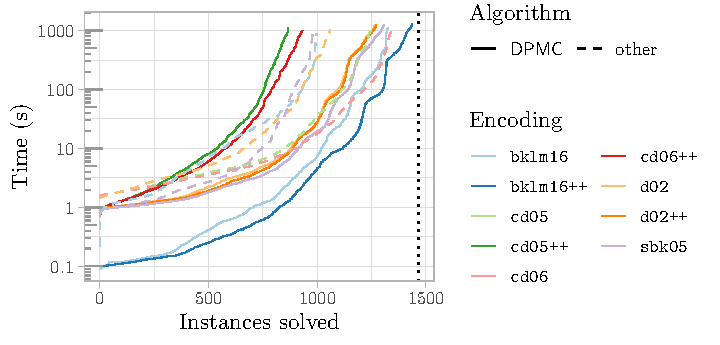
\includegraphics[width=\textwidth]{chapters/wmc_without_parameters/cumulative}
  \caption{Cactus plot of all algorithm-encoding pairs. The dotted line denotes
    the total number of instances used.}\label{fig:cumulative2}
\end{figure}

\begin{figure}[t]
  \centering
  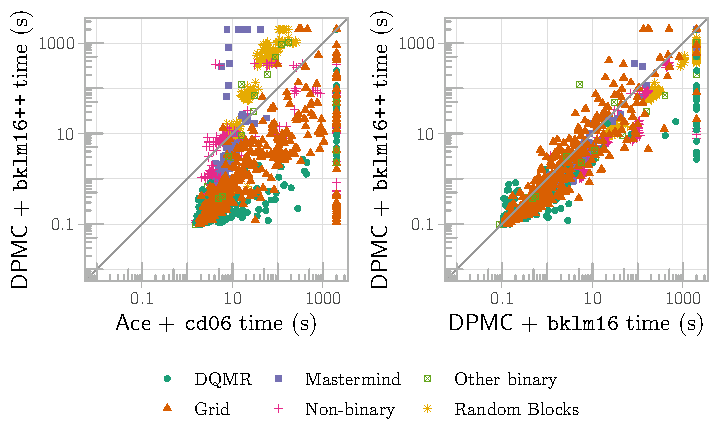
\includegraphics[width=\textwidth]{chapters/wmc_without_parameters/scatter}
  \caption{An instance-by-instance comparison between $\textsc{DPMC} +
    \texttt{bklm16++}$ (the best combination according to \cref{fig:cumulative2})
  and the second and third best-performing combinations: $\textsc{Ace} +
  \texttt{cd06}$ and $\textsc{DPMC} + \texttt{bklm16}$.}\label{fig:scatter2}
\end{figure}

\begin{figure}[t]
  \centering
  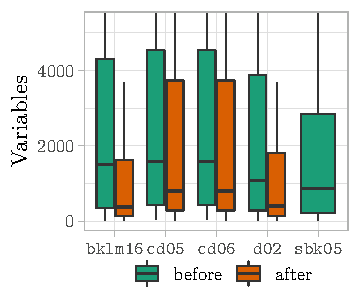
\includegraphics[width=\textwidth]{chapters/wmc_without_parameters/box}
  \caption{Box plots of the numbers of variables in each encoding across all
    benchmark instances before and after applying \cref{alg:transformation}.
    Outliers and the top parts of some whiskers are omitted.}\label{fig:box}
\end{figure}

\begin{table}[t]
  \centering
  \begin{tabular}{lrr}
    \toprule
    Combination & Fastest & Solved \\
    \midrule
    $\textsc{Ace} + \texttt{cd05}$ & 27 & 1247 \\
    $\textsc{Ace} + \texttt{cd06}$ & 135 & 1340 \\
    $\textsc{Ace} + \texttt{d02}$ & 56 & 1060 \\
    $\textsc{DPMC} + \texttt{bklm16}$ & 241 & 1327 \\
    $\textsc{DPMC} + \texttt{bklm16++}$ & \textbf{992} & \textbf{1435} \\
    $\textsc{DPMC} + \texttt{cd05++}$ & \textcolor{gray}{0} & 867 \\
    $\textsc{DPMC} + \texttt{cd06++}$ & \textcolor{gray}{0} & 932 \\
    $\textsc{DPMC} + \texttt{d02}$ & 1 & 1267 \\
    $\textsc{DPMC} + \texttt{d02++}$ & 7 & 1272 \\
    $\textsc{DPMC} + \texttt{sbk05}$ & 31 & 1308 \\
    $\textsc{c2d} + \texttt{bklm16}$ & \textcolor{gray}{0} & 997 \\
    $\textsc{Cachet} + \texttt{sbk05}$ & 49 & 983 \\
    \bottomrule
  \end{tabular}
  \caption{The numbers of instances (out of 1466) that each algorithm and
    encoding combination solved faster than any other combination and in
    total.}\label{tbl:performance}
\end{table}

\Cref{fig:cumulative2} shows $\textsc{DPMC}+\texttt{bklm16++}$ to be the
best-performing combination across all time limits up to \SI{1000}{\second} with
$\textsc{Ace} + \texttt{cd06}$ and $\textsc{DPMC}+\texttt{bklm16}$ not far
behind. Overall, $\textsc{DPMC}+\texttt{bklm16++}$ is 3.35 times faster than
$\textsc{DPMC}+\texttt{bklm16}$ and 2.96 times faster than
$\textsc{Ace}+\texttt{cd06}$. \Cref{tbl:performance} further shows that
$\textsc{DPMC}+\texttt{bklm16++}$ solves almost a hundred more instances than
any other combination, and is the fastest in \SI{69.1}{\percent} of them.

The scatter plots in \cref{fig:scatter2} show that how $\textsc{DPMC} +
\texttt{bklm16++}$ (and perhaps \textsc{DPMC} more generally) compares to
$\textsc{Ace} + \texttt{cd06}$ depends significantly on the data set: the former
is a clear winner on DQMR and Grid instances, while the latter performs well on
Mastermind and Random Blocks. Perhaps because the underlying WMC algorithm
remains the same, the difference between $\textsc{DPMC} + \texttt{bklm16}$ with
and without applying \cref{alg:transformation} is quite noisy, i.e, with most
instances scattered around the line of equality. However, our transformation
does enable \textsc{DPMC} to solve many instances that were previously beyond
its reach.

We also record numbers of variables in each encoding before and after applying
\cref{alg:transformation}. \Cref{fig:box} shows a significant reduction in the
number of variables. For instance, the median number of variables in instances
encoded with \texttt{bklm16} was reduced four times: from 1499 to 376. While
\texttt{bklm16++} results in the overall lowest number of variables, the
difference between \texttt{bklm16++} and \texttt{d02++} seems small. Indeed, the
numbers of variables in these two encodings are equal for binary Bayesian
networks (i.e., most of our data). Nonetheless, \texttt{bklm16++} is still much
faster than \texttt{d02++} when run with \textsc{DPMC}.

It is also worth noting that there was no observable difference in the width of
the project-join tree used by \textsc{DPMC} (which is equivalent to the primal
treewidth of the input formula \citep{DBLP:conf/cp/DudekPV20}) before and after
applying \cref{alg:transformation}---the observed performance improvement is
more likely related to the variable ordering heuristic used by
ADDs.\footnote{The data on this (along with the implementation of
  \cref{alg:transformation}) is available at
  \url{https://github.com/dilkas/wmc-without-parameters}.}

Overall, transforming WMC instances to the PBP format allows us to significantly
simplify each instance. This transformation is particularly effective on
\texttt{bklm16}, allowing it to surpass \texttt{cd06} and become the new state
of the art. While there is a similarly significant reduction in the number of
variables for \texttt{d02}, the performance of $\textsc{DPMC}+\texttt{d02}$ is
virtually unaffected. Finally, while our transformation makes it possible to use
\texttt{cd05} and \texttt{cd06} with \textsc{DPMC}, the two combinations remain
inefficient.

\section{Conclusion and Future Work}

In this chapter, we showed how the number of variables in a WMC instance can be
significantly reduced by transforming it into a representation based on
two-valued pseudo-Boolean functions. In some cases, this led to significant
improvements in inference speed, allowing $\textsc{DPMC} + \texttt{bklm16++}$ to
overtake $\textsc{Ace}+\texttt{cd06}$ as the new state of the art WMC technique
for Bayesian network inference. Moreover, we identified key properties of
Bayesian network encodings that allow for parameter variable removal. However,
these properties were rather different for each encoding, and so an interesting
question for future work is whether they can be unified into a more abstract and
coherent list of conditions.

Bayesian network inference was chosen as the example application of WMC because
it is the first and the most studied one
\citep{DBLP:conf/ecai/BartKLM16,DBLP:conf/ijcai/ChaviraD05,DBLP:conf/sat/ChaviraD06,DBLP:conf/kr/Darwiche02,DBLP:conf/aaai/SangBK05}.
While the distinction between indicator and parameter variables is often not
explicitly described in other WMC encodings
\citep{DBLP:journals/tplp/FierensBRSGTJR15,DBLP:journals/pacmpl/HoltzenBM20,DBLP:conf/icml/XuZFLB18},
perhaps variables could still be partitioned in this way, allowing for not just
faster inference with \textsc{DPMC} or \textsc{ADDMC} but also for
well-established WMC encoding and inference techniques (such as in the work by
\citet{DBLP:conf/ijcai/ChaviraD05,DBLP:conf/sat/ChaviraD06}) to be transferred
to other application domains.

Similarly, could weighted first-order model counting (WFOMC) benefit from a more
flexible approach to weights? The standard (`symmetric') definition of WFOMC
assigns a pair of weights to each predicate
\citep{DBLP:conf/ijcai/BroeckTMDR11}. Perhaps WFOMC could benefit from weights
that depend on numerical constants in addition to predicates. This idea could
also be seen as an extension of weighted first-order model integration
\citep{DBLP:conf/uai/FeldsteinB21} to discrete measurable spaces.

Lastly, we noted how the parameter equivalent to primal treewidth used by
\textsc{DPMC} \citep{DBLP:conf/cp/DudekPV20} remains virtually unchanged by our
transformation despite a significant reduction in instance size. We also know
that WMC (and hence WMC in the PBP format) is fixed-parameter tractable (FPT)
with respect to primal treewidth (see \cref{chapter:comparison} for a discussion
on the parameterised complexity of WMC). WMC being FPT means that it admits
\emph{kernelisation}. In other words, any WMC instance can be transformed (in
polynomial time) to an instance whose size depends only on the parameter (e.g.,
primal treewidth) and not on the size of the original instance
\citep{DBLP:series/txcs/DowneyF13}. So, perhaps the WMC to PBP transformation
presented in this chapter can be improved and formalised into a kernelisation
algorithm for WMC instances within this more flexible PBP format. Kernelisation
as well as the parameterised complexity angle on WMC more broadly is an
underexplored area of research that we approach in more detail in
\cref{chapter:comparison}.

% What are the directions for the future present themselves that you have not investigated in this thesis?
% What other lessons can you draw?
